% ================= APPENDIX: ELECTRICAL SYSTEM DETAIL =================
\section{Electrical System Detail}
\label{app:electrical}

This appendix holds the electrical detail kept out of
Section~\ref{sec:electrical}: the schematic sheets indexed in
Table~\ref{tab:schematic_sheets}, the connector and pin assignments, the harness
drawings, the board layout and the bring-up checklists. The architectural
decisions --- two rails behind one E-stop, linear bus topology, perfboard rather
than fabricated board --- remain in Section~\ref{sec:electrical}. The part
specifications are in Appendix~\ref{app:bom} and are not repeated.

\subsection{Schematic Sheets}
\label{app:schematics}
\label{app:schematic_full}

The system is captured on one flat KiCad sheet, reproduced at page size in
Figure~\ref{fig:schematic_full} and listed by functional block in
Table~\ref{tab:schematic_sheets}. That capture is the working drawing the build
is wired from. The blocks it carries are: power entry and protection (pack
connector, anti-spark inrush path, combined E-stop and fuse, split to the motor
bus and the logic rail); the \qty{5}{\volt} logic rail off an LM2596 converter
with back-feed protection and per-device decoupling; the CAN-FD bus as a linear
chain across the three moteus drivers and the flight computer, terminated at
the two physical ends only; the per-axis encoder SPI interfaces; the Teensy 4.1
flight computer with the BMI270 IMU; the ESP32 telemetry link; and the three
brake servo drives.

Note: for the provided N35 $1/4" \times 1/8"$ diametric disk magnet, the optimal
distance in order to achieve the \qty{20}{\milli\tesla} --
\qty{80}{\milli\tesla} nominal magnetic field for the MA600 encoder is
\qty{3.3}{\milli\metre}.

The per-block schematic sheets, split out of this capture as a release step
rather than a redraw, are to be added in the final draft.

% ---------------------------------------------------------------------------
% Per-sheet figures, split out of images/schematic_full.pdf as a release step
% (not a redraw: the sheets must agree with the capture net for net). Each is
% followed by a per-pin electrical/logic table -- net name, direction, level
% and function -- so the sheet can be wired from this document without a
% KiCad viewer. Physical pin numbers are marked TBD where they depend on the
% board layout of Section~\ref{sec:layout}, which is not yet drawn; the net
% identity, direction and level are fixed by the architecture of
% Section~\ref{sec:electrical} and are not TBD.

\subsubsection{Sheet 1 --- Power Entry and Protection}
\begin{figure}[htbp]
\centering
\phfig[0.30\textheight]{0.82\textwidth}{Schematic sheet 1 --- power entry and protection:
pack connector, anti-spark inrush path, combined E-stop and fuse, and the split
to the motor bus and the logic rail.}
\caption[Schematic sheet 1: power entry and protection]{Schematic sheet 1 --- power entry and protection. To be verified
against the fuse rating vs.\ worst-case bus current
(Table~\ref{tab:power_budget}) and the inrush into the driver bulk
capacitance.}
\label{fig:sch_power_entry}
\end{figure}

\begin{table}[htbp]
\centering
\caption[Sheet 1 pin/net logic]{Sheet 1 pin/net logic. Connector refs are J1--J2 of Table~\ref{tab:connectors}.}
\label{tab:pins_power_entry}
\small
\setlength{\tabcolsep}{4pt}
\begin{tabular}{c L{2.6cm} c L{2.4cm} L{5.4cm}}
\toprule
Pin & Net & Direction & Level & Function \\
\midrule
J1-1 & PACK+ & In & \qty{22.2}{\volt} nominal (6S) & Battery positive, upstream of E-stop and fuse \\
J1-2 & PACK$-$ & In & 0\,V (system return) & Battery negative \\
\textcolor{red}{TBD} & ESTOP\_SENSE & In & Switched PACK+ & E-stop contact; open interrupts the bus, not a logic signal \\
\textcolor{red}{TBD} & FUSE & In/Out & Switched PACK+ & Series fuse element, motor-bus rated \\
J2-1 & MOTOR\_BUS+ & Out & \qtyrange{22}{25}{\volt} (discharge curve) & To distribution board, motor bus (Sec.~\ref{sec:power_arch}) \\
J2-2 & MOTOR\_BUS$-$ & Out & 0\,V (system return) & Motor bus return \\
\bottomrule
\end{tabular}
\end{table}

\subsubsection{Sheet 2 --- Logic Rail}
\begin{figure}[htbp]
\centering
\phfig[0.30\textheight]{0.82\textwidth}{Schematic sheet 2 --- \qty{5}{\volt} logic rail:
buck converter, back-feed protection diode, rail bulk capacitance and
per-device decoupling.}
\caption[Schematic sheet 2: logic rail]{Schematic sheet 2 --- \qty{5}{\volt} logic rail. To be verified against
the converter rating vs.\ the worst-case rail total, and against capacitor
voltage ratings by position: low-voltage parts on the logic rail only, never on
the pack bus.}
\label{fig:sch_logic_rail}
\end{figure}

\begin{table}[htbp]
\centering
\caption[Sheet 2 pin/net logic]{Sheet 2 pin/net logic (LM2596 buck converter).}
\label{tab:pins_logic_rail}
\small
\setlength{\tabcolsep}{4pt}
\begin{tabular}{c L{2.6cm} c L{2.4cm} L{5.4cm}}
\toprule
Pin & Net & Direction & Level & Function \\
\midrule
\textcolor{red}{TBD} & VIN & In & \qtyrange{22}{25}{\volt} & Converter input, tapped off MOTOR\_BUS+ upstream of the motor drivers \\
\textcolor{red}{TBD} & GND & In/Out & 0\,V & Converter ground, common with system return \\
\textcolor{red}{TBD} & VOUT (5V\_LOGIC) & Out & \qty{5.00}{\volt} $\pm$\qty{0.05}{\volt} & Logic rail feed, back-fed through a series diode into the rail bus \\
\textcolor{red}{TBD} & EN & In & 3.3--5\,V logic & Converter enable, tied to the E-stop chain \\
\bottomrule
\end{tabular}
\end{table}

\subsubsection{Sheet 3 --- CAN-FD Bus}
\begin{figure}[htbp]
\centering
\phfig[0.30\textheight]{0.82\textwidth}{Schematic sheet 3 --- CAN-FD bus:
linear chain across the three drivers and the flight computer, with split
termination at the two physical ends.}
\caption[Schematic sheet 3: CAN-FD bus]{Schematic sheet 3 --- CAN-FD bus. To be verified against the topology
rules of Table~\ref{tab:signal_rules}: linear chain, bounded stubs, termination
at the two physical ends only.}
\label{fig:sch_can_bus}
\end{figure}

\begin{table}[htbp]
\centering
\caption[Sheet 3 pin/net logic]{Sheet 3 pin/net logic. J6/J7 are the chain-end connectors of
Table~\ref{tab:connectors}; each moteus driver and the flight computer tap the
chain as a short stub, per Section~\ref{sec:bus_topology}.}
\label{tab:pins_can_bus}
\small
\setlength{\tabcolsep}{4pt}
\begin{tabular}{c L{2.6cm} c L{2.4cm} L{5.4cm}}
\toprule
Pin & Net & Direction & Level & Function \\
\midrule
J6-1 / J7-1 & CAN\_H & Bidir, differential & \qty{2.5}{\volt} $\pm$ swing & Bus high, chain end A / end B \\
J6-2 / J7-2 & CAN\_L & Bidir, differential & \qty{2.5}{\volt} $\mp$ swing & Bus low, chain end A / end B \\
J6-3 / J7-3 & GND & In/Out & 0\,V & Bus reference, common return (Sec.~\ref{sec:bus_topology}) \\
\textcolor{red}{TBD} & $R_{\text{term}}$ (end A, end B) & --- & \qty{120}{\ohm} each & Termination, two physical ends only; \qty{60}{\ohm} $\pm$\qty{3}{\ohm} unpowered across CAN\_H--CAN\_L (Sec.~\ref{sec:elec_checks}) \\
\bottomrule
\end{tabular}
\end{table}

\subsubsection{Sheet 4 --- Encoder Interfaces}
\begin{figure}[htbp]
\centering
\phfig[0.30\textheight]{0.82\textwidth}{Schematic sheet 4 --- encoder interfaces:
the SPI interface from driver to encoder, one instance per axis, with the
air-gap dimension called out.}
\caption[Schematic sheet 4: encoder interfaces]{Schematic sheet 4 --- encoder interfaces ($3\times$). To be verified
against the SPI cable length limit and the \qty{3.3}{\milli\metre} air gap; these
fix the driver positions rather than the reverse
(Sec.~\ref{sec:bus_topology}).}
\label{fig:sch_encoders}
\end{figure}

\begin{table}[htbp]
\centering
\caption[Sheet 4 pin/net logic]{Sheet 4 pin/net logic, per axis $i\in\{1,2,3\}$. Connector J8 of
Table~\ref{tab:connectors}; MA600 encoder SPI, one instance per moteus driver.}
\label{tab:pins_encoders}
\small
\setlength{\tabcolsep}{4pt}
\begin{tabular}{c L{2.6cm} c L{2.4cm} L{5.4cm}}
\toprule
Pin & Net & Direction & Level & Function \\
\midrule
J8-1 & MOSI\_$i$ & Out (driver$\to$encoder) & \qty{3.3}{\volt} logic & SPI data to encoder \\
J8-2 & MISO\_$i$ & In (encoder$\to$driver) & \qty{3.3}{\volt} logic & SPI data from encoder (absolute angle) \\
J8-3 & SCK\_$i$ & Out (driver$\to$encoder) & \qty{3.3}{\volt} logic & SPI clock \\
J8-4 & CS\_$i$ & Out (driver$\to$encoder) & \qty{3.3}{\volt} logic & SPI chip select, active low \\
J8-5 & 3V3 & Out (driver$\to$encoder) & \qty{3.3}{\volt} & Encoder supply \\
J8-6 & GND & In/Out & 0\,V & Encoder return \\
\bottomrule
\end{tabular}
\end{table}

\subsubsection{Sheet 5 --- Flight Computer and IMU}
\begin{figure}[htbp]
\centering
\phfig[0.30\textheight]{0.82\textwidth}{Schematic sheet 5 --- flight computer and IMU:
MCU, IMU interface, and the sensor orientation relative to the body frame.}
\caption[Schematic sheet 5: flight computer and IMU]{Schematic sheet 5 --- flight computer and IMU. To be verified against
the sensor orientation relative to the body frame of
Sec.~\ref{sec:cad_method} and the mounting location relative to the pivot
required by Sec.~\ref{sec:control_algorithms}.}
\label{fig:sch_fc_imu}
\end{figure}

\begin{table}[htbp]
\centering
\caption[Sheet 5 pin/net logic]{Sheet 5 pin/net logic. Connector J9 of Table~\ref{tab:connectors};
Teensy~4.1 to BMI270, plus the CAN-FD transceiver interface consumed by
Sheet~3.}
\label{tab:pins_fc_imu}
\small
\setlength{\tabcolsep}{4pt}
\begin{tabular}{c L{2.6cm} c L{2.4cm} L{5.4cm}}
\toprule
Pin & Net & Direction & Level & Function \\
\midrule
J9-1 & IMU\_MOSI & Out (Teensy$\to$IMU) & \qty{3.3}{\volt} logic & SPI data to BMI270 \\
J9-2 & IMU\_MISO & In (IMU$\to$Teensy) & \qty{3.3}{\volt} logic & SPI data from BMI270 \\
J9-3 & IMU\_SCK & Out (Teensy$\to$IMU) & \qty{3.3}{\volt} logic & SPI clock \\
J9-4 & IMU\_CS & Out (Teensy$\to$IMU) & \qty{3.3}{\volt} logic & SPI chip select, active low \\
J9-5 & IMU\_INT & In (IMU$\to$Teensy) & \qty{3.3}{\volt} logic & Data-ready interrupt, sampled each \qty{1}{\milli\second} tick (Sec.~\ref{sec:software_pipeline}) \\
J9-6 & 3V3 / GND & Out / In-Out & \qty{3.3}{\volt} / 0\,V & IMU supply and return \\
\textcolor{red}{TBD} & CAN\_TX / CAN\_RX & Out / In & \qty{3.3}{\volt} logic (to transceiver) & Teensy CAN-FD peripheral to the bus transceiver of Sheet~3 \\
\bottomrule
\end{tabular}
\end{table}

\subsubsection{Sheet 6 --- Telemetry Link}
\begin{figure}[htbp]
\centering
\phfig[0.30\textheight]{0.82\textwidth}{Schematic sheet 6 --- telemetry link:
telemetry module, serial interface to the MCU, and the supply decoupling sized
for the transmit burst.}
\caption[Schematic sheet 6: telemetry link]{Schematic sheet 6 --- telemetry link. To be verified against the
transmit-burst current and its return path off the logic rail.}
\label{fig:sch_telemetry}
\end{figure}

\begin{table}[htbp]
\centering
\caption[Sheet 6 pin/net logic]{Sheet 6 pin/net logic. Connector J10 of Table~\ref{tab:connectors};
Teensy~4.1 to the XIAO ESP32-C6 telemetry module.}
\label{tab:pins_telemetry}
\small
\setlength{\tabcolsep}{4pt}
\begin{tabular}{c L{2.6cm} c L{2.4cm} L{5.4cm}}
\toprule
Pin & Net & Direction & Level & Function \\
\midrule
J10-1 & UART\_TX & Out (Teensy$\to$ESP32) & \qty{3.3}{\volt} logic & Telemetry data to the ESP32 \\
J10-2 & UART\_RX & In (ESP32$\to$Teensy) & \qty{3.3}{\volt} logic & Command/ack path from the ESP32 \\
J10-3 & 5V\_LOGIC & Out (board$\to$ESP32) & \qty{5.00}{\volt} & ESP32 supply, sized for the \qty{300}{\milli\ampere} transmit burst (Table~\ref{tab:electrical_criteria}) \\
J10-4 & GND & In/Out & 0\,V & Return \\
\bottomrule
\end{tabular}
\end{table}

\subsubsection{Sheet 7 --- Brake Servo Drive}
\begin{figure}[htbp]
\centering
\phfig[0.30\textheight]{0.82\textwidth}{Schematic sheet 7 --- brake servo drive:
servo supply, decoupling and PWM routing, one instance per axis.}
\caption[Schematic sheet 7: brake servo drive]{Schematic sheet 7 --- brake servo drive. To be verified against
stall-current headroom on the logic rail, with the PWM routed clear of the
encoder SPI.}
\label{fig:sch_servo}
\end{figure}

\begin{table}[htbp]
\centering
\caption[Sheet 7 pin/net logic]{Sheet 7 pin/net logic, per axis $i\in\{1,2,3\}$. Connector J11 of
Table~\ref{tab:connectors}; TowerPro MG92B brake servos.}
\label{tab:pins_servo}
\small
\setlength{\tabcolsep}{4pt}
\begin{tabular}{c L{2.6cm} c L{2.4cm} L{5.4cm}}
\toprule
Pin & Net & Direction & Level & Function \\
\midrule
J11-1 & PWM\_$i$ & Out (Teensy$\to$servo) & \qty{3.3}{\volt} logic, \qty{50}{\hertz} & Servo position command, routed clear of the encoder SPI runs of Sheet~4 \\
J11-2 & 5V\_LOGIC & Out (board$\to$servo) & \qty{5.00}{\volt} & Servo supply \\
J11-3 & GND & In/Out & 0\,V & Servo return; flyback path verified per Table~\ref{tab:electrical_criteria} \\
\bottomrule
\end{tabular}
\end{table}
% ---------------------------------------------------------------------------

% The full schematic is drawn on its own landscape page rather than scaled into
% the text block: reduced to \textwidth in portrait the reference designators
% and net labels fall below legibility. Same treatment as the Gantt sheets of
% Sec. 2 -- see sections/02_project_organization_gantt.tex.
%
% Source: images/schematic_full.pdf, a single-page A4 landscape vector export
% from KiCad (a copy of "Circuit Schematic - Classic Color.pdf", renamed because
% \includegraphics does not take spaces in a path). Re-export over that file to
% update the sheet; no edit here is needed. On a landscape page \linewidth is the
% long edge, so the height limit is expressed in \textwidth -- with
% keepaspectratio, whichever bound binds first is the one applied.

% Empty page style for the rotated sheet: the running header and footer would
% otherwise be typeset sideways along the page edge.
\fancypagestyle{cublischematic}{%
  \fancyhf{}%
  \renewcommand{\headrulewidth}{0pt}%
  \renewcommand{\footrulewidth}{0pt}%
}

\begin{landscape}
\pagestyle{cublischematic}
\begin{figure}[p]
\thispagestyle{cublischematic}
\centering
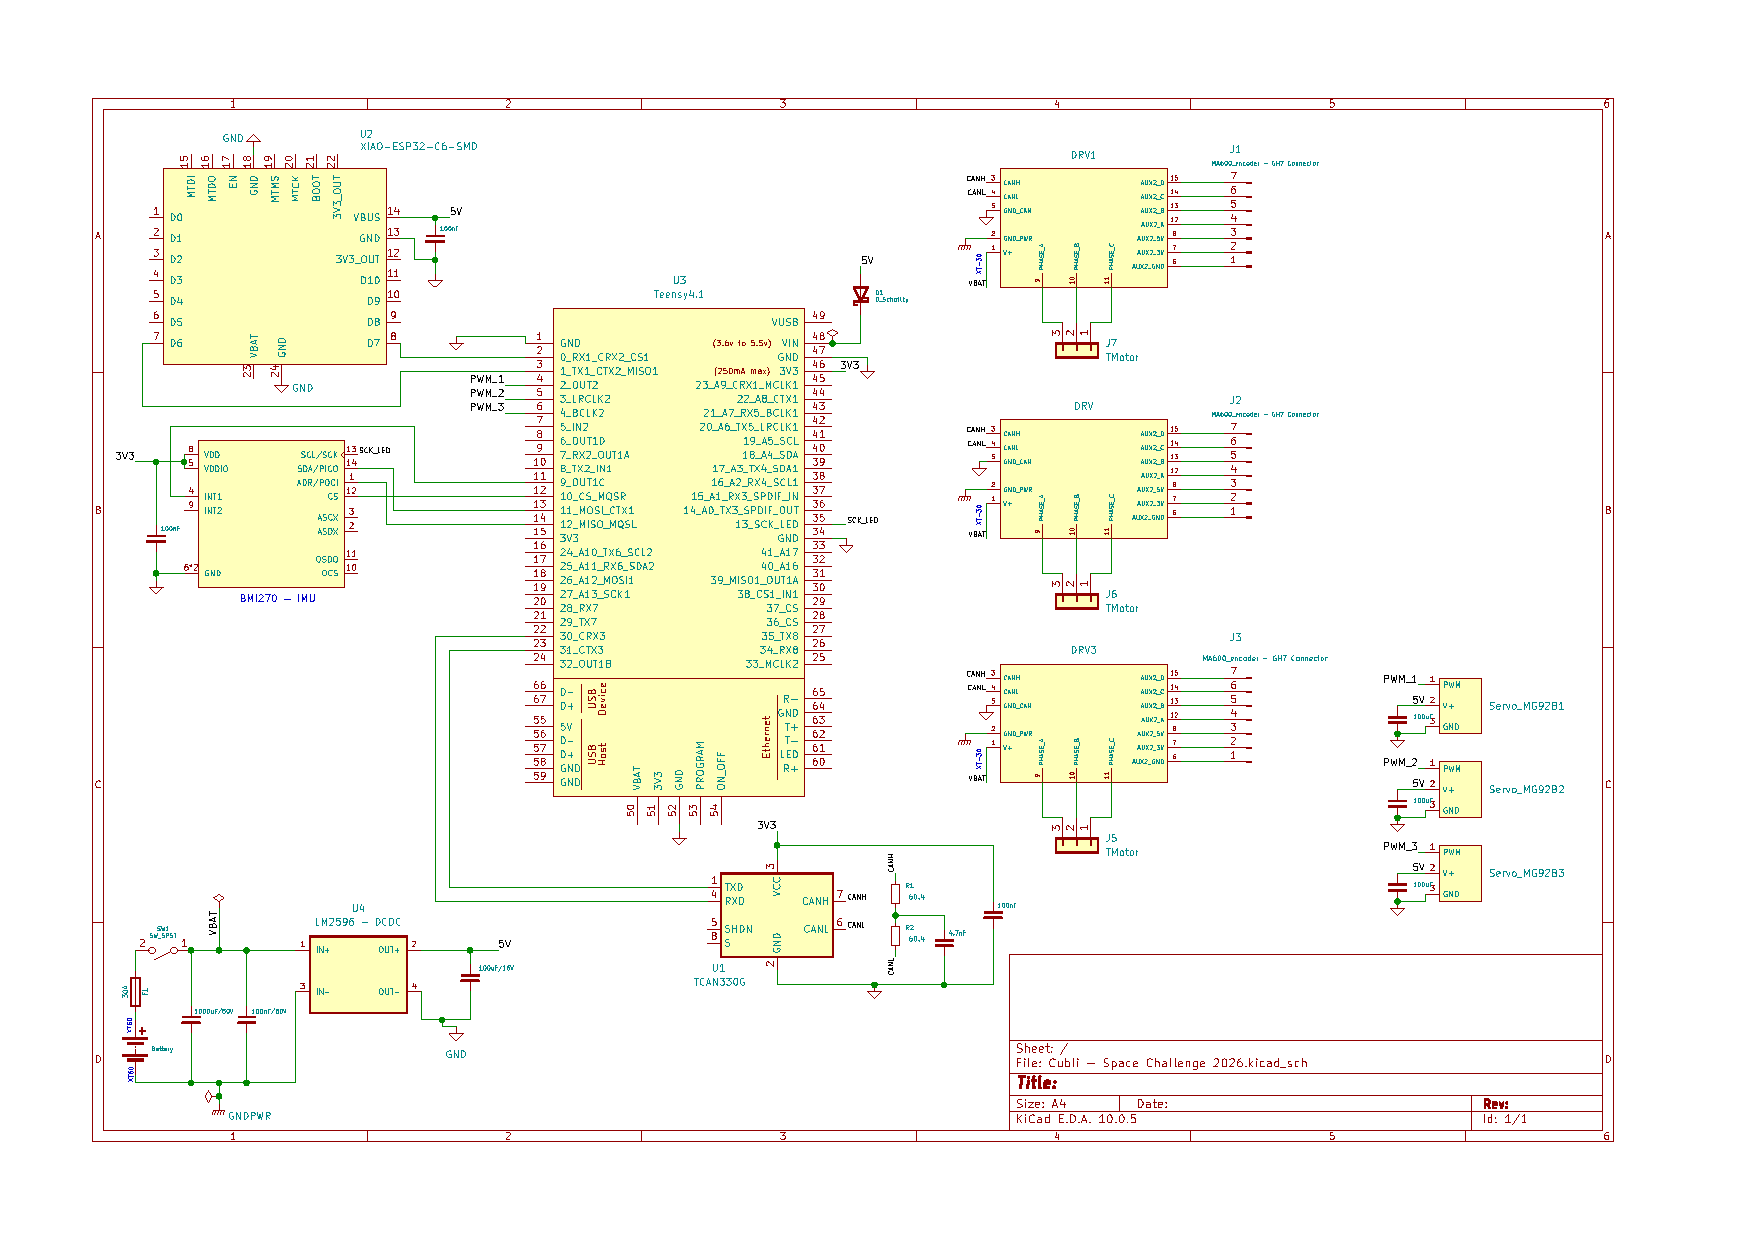
\includegraphics[width=\linewidth,height=1.0\textwidth,keepaspectratio]{images/schematic_full.pdf}
\caption[Full electrical schematic (landscape sheet)]{Full electrical schematic as captured, reproduced at page size.
Covers the flight computer (Teensy 4.1) and its ESP32 telemetry module, the
BMI270 IMU, the three moteus driver and motor connectors, the CAN-FD
transceiver and termination, the LM2596 \qty{5}{\volt} converter from the pack,
and the three brake servos. The per-block sheets are drawn from this capture as
it is split for release.}
\label{fig:schematic_full}
\end{figure}
\end{landscape}
\pagestyle{fancy}

\subsection{Connector and Pin Assignments}
\label{app:pinout}

Table~\ref{tab:connectors} is the connector schedule. It exists so that a
harness can be built and re-built from this document alone, and so that a
mis-mate is a documented impossibility rather than a discovered one: no two
connectors carrying different voltages share a housing type on this machine.

\begin{table}[htbp]
\centering
\caption[Connector schedule]{Connector schedule. Keying and housing types are chosen so that two
connectors carrying different voltages cannot be mated. Note: values have not been finalized at this preliminary stage. }
\label{tab:connectors}
\small
\setlength{\tabcolsep}{4pt}
\begin{tabular}{c L{3.0cm} L{3.0cm} L{2.4cm} L{3.2cm}}
\toprule
Ref & From & To & Housing / keying & Signals \\
\midrule
J1 & Battery pack        & Protection / E-stop   & \textcolor{red}{TBD} & Pack $+$, pack $-$ \\
J2 & Protection          & Distribution board    & \textcolor{red}{TBD} & Motor bus \\
J3 & Distribution board  & Driver, axis 1        & \textcolor{red}{TBD} & Motor bus \\
J4 & Distribution board  & Driver, axis 2        & \textcolor{red}{TBD} & Motor bus \\
J5 & Distribution board  & Driver, axis 3        & \textcolor{red}{TBD} & Motor bus \\
J6 & Board               & CAN chain, end A      & \textcolor{red}{TBD} & CAN-H, CAN-L, GND \\
J7 & CAN chain, end B    & Termination network   & \textcolor{red}{TBD} & CAN-H, CAN-L, GND \\
J8 & Driver, axis $i$    & Encoder, axis $i$     & \textcolor{red}{TBD} & SPI, \qty{3.3}{\volt}, GND \\
J9 & Board               & IMU                   & \textcolor{red}{TBD} & Serial bus, supply, GND \\
J10 & Board              & Telemetry module      & \textcolor{red}{TBD} & UART, supply, GND \\
J11 & Board              & Brake servo, axis $i$ & \textcolor{red}{TBD} & PWM, \qty{5}{\volt}, GND \\
\bottomrule
\end{tabular}
\end{table}

\subsection{Harness Drawings and Wire Schedule}
\label{app:harness}

Table~\ref{tab:wire_schedule} is the wire schedule. Conductor gauge on the motor
bus is set by the spin-up current rather than the balancing current, since
spin-up is the sustained high-current phase; the signal runs are set by length
limits rather than by current.

\begin{table}[htbp]
\centering
\caption[Wire schedule]{Wire schedule. Motor-bus gauge is sized on spin-up current; signal runs
are length-limited (Table~\ref{tab:signal_rules}). Note: values have not been finalized at this preliminary stage. }
\label{tab:wire_schedule}
\small
\setlength{\tabcolsep}{4pt}
\begin{tabular}{c L{3.4cm} c c L{3.8cm}}
\toprule
Ref & Run & Gauge & Length & Sizing basis \\
\midrule
H1 & Pack to protection      & \textcolor{red}{TBD} & \textcolor{red}{TBD} & Peak bus current \\
H2 & Protection to board     & \textcolor{red}{TBD} & \textcolor{red}{TBD} & Peak bus current \\
H3 & Board to driver drops (3) & \textcolor{red}{TBD} & \textcolor{red}{TBD} & Per-axis spin-up current \\
H4 & Motor phase leads (3)   & \textcolor{red}{TBD} & \textcolor{red}{TBD} & Motor phase current \\
H5 & CAN chain segments      & \textcolor{red}{TBD} & \textcolor{red}{TBD} & Topology, not current \\
H6 & Encoder SPI runs (3)    & \textcolor{red}{TBD} & \textcolor{red}{TBD} & Length limit governs \\
H7 & Servo drives (3)        & \textcolor{red}{TBD} & \textcolor{red}{TBD} & Stall current \\
\bottomrule
\end{tabular}
\end{table}

% Figure placeholder: distribution harness drawing -- pack lead, protection
% element, and the three driver drops, with labelling scheme.
% Figure placeholder: as-built harness photograph, labelled and strain-relieved.

\subsection{Board Layout}
\label{app:board_layout}

% Figure placeholder: perfboard floorplan -- bus entry, converter, logic rail,
% bulk capacitance, flight computer, IMU, telemetry module, servo headers and
% the CAN termination network.
% Figure placeholder: board outline drawing with the mounting-hole pattern,
% keep-out heights and connector exit directions delivered to the mechanical
% design as the electronics-mount interface of Table~\ref{tab:mech_interfaces}.

The floorplan is constrained before it is aesthetic: the driver positions follow
from the encoder cable limit, the bus route follows from the driver positions,
and the board is placed around what remains
(Section~\ref{sec:bus_topology}). Rail separation is maintained physically on
the board, not only schematically, so that motor-current return does not share
copper with the sensing ground.

\subsection{Bring-Up and Isolation Checklists}
\label{app:checklists}

These checks are performed on every re-assembly, not only on first build, since
the encoder gaps and connector seating are exactly what mechanical work
disturbs.

\paragraph{Before any power is applied.}
\begin{enumerate}
  \item Isolation: motor bus to chassis, logic rail to motor bus, each rail to
        ground.
  \item Capacitor voltage ratings confirmed by position --- no low-voltage part
        on the pack bus.
  \item Polarity of every fabricated connector verified against
        Table~\ref{tab:connectors}.
  \item Protection element in circuit: E-stop functional, fuse fitted and rated,
        anti-spark path intact.
  \item Encoder air gaps re-measured after mechanical assembly.
\end{enumerate}

\paragraph{First power-on, current-limited bench supply.}
\begin{enumerate}
  \item Current limit verified against a known load before connecting the
        assembly.
  \item Logic rail voltage and ripple under load; converter thermal check.
  \item All drivers enumerate on the bus; encoders read back with no error
        flags; IMU responds.
  \item Bus integrity at the full data rate: sustained soak with all nodes
        addressed, error-frame count logged.
  \item Open-loop wheel motion, wheels contained, one axis at a time.
\end{enumerate}

\paragraph{First battery power-on.} Performed only after the bench sequence
passes in full, with the pack protection verified, cell monitoring active and
the assembly in a fire-safe area. Inrush is measured against the bulk
capacitance on connection.

\subsection{As-Built Measurements}
\label{app:electrical_measured}

Table~\ref{tab:electrical_measured} records the measured electrical figures that
replace the estimates used during design. These are the numbers reported back to
the modelling and control work, and they are the reason the parameter
identification of Section~\ref{sec:paramid} runs on measured rather than assumed
values.

\begin{table}[htbp]
\centering
\caption[As-built electrical measurements]{As-built electrical measurements. Each replaces an estimate used
earlier in the design. Note: values have not been finalized at this preliminary stage. }
\label{tab:electrical_measured}
\small
\begin{tabular}{L{5.0cm} c L{5.4cm}}
\toprule
Quantity & Measured & Replaces / feeds \\
\midrule
Motor torque constant $K_m$    & \textcolor{red}{TBD} & Table~\ref{tab:params}, datasheet value \\
Wheel inertia $I_w$ (spin-down)& \textcolor{red}{TBD} & Table~\ref{tab:params}, CAD value \\
Viscous and Coulomb friction   & \textcolor{red}{TBD} & $C_b$, $C_w$ estimates \\
Command-to-encoder latency     & \textcolor{red}{TBD} & Loop timing, Sec.~\ref{sec:control_sw} \\
Achievable wheel speed on bus  & \textcolor{red}{TBD} & $\omega_{\max}$, Sec.~\ref{sec:jumpup_target} \\
Logic rail load, worst case    & \textcolor{red}{TBD} & Table~\ref{tab:power_budget} \\
Runtime per charge under balance load & \textcolor{red}{TBD} & Demonstration planning \\
\bottomrule
\end{tabular}
\end{table}
